
%%%%%%%%%%%%%%%%%%%%%%%%%%%%%%  IEEEsample2e.tex %%%%%%%%%%%%%%%%%%%%%%%%%%%%%%
%% changes for IEEEtrans.cls marked with !PN
%% except all occ. of IEEEtran.sty changed IEEEtran.cls
%%%%%%%%%%                                                       %%%%%%%%%%%%%
%%%%%%%%%%    More information: see the header of IEEEtran.cls   %%%%%%%%%%%%%
%%%%%%%%%%                                                       %%%%%%%%%%%%%
%%%%%%%%%%%%%%%%%%%%%%%%%%%%%%%%%%%%%%%%%%%%%%%%%%%%%%%%%%%%%%%%%%%%%%%%%%%%%%%

\documentclass[journal,transmag]{IEEEtran}
\usepackage[portuguese]{babel}
%\documentclass[twocolumn]{IEEEtran} %!PN
%\documentclass[12pt,draft]{IEEEtran} %!PN
%\documentstyle[twocolumn]{IEEEtran}
%\documentstyle[12pt,twoside,draft]{IEEEtran}
%\documentstyle[9pt,twocolumn,technote,twoside]{IEEEtran}
\usepackage{graphicx}
\usepackage{amsmath}
%\graphicspath{{../figures/}{fig_site/}}

\def\BibTeX{{\rm B\kern-.05em{\sc i\kern-.025em b}\kern-.08em
    T\kern-.1667em\lower.7ex\hbox{E}\kern-.125emX}}

\newtheorem{theorem}{Theorem}
\setcounter{page}{1}

\begin{document}

%\title{Using the Style File IEEEtran.sty} 
\title{Ultralytics YOLO: Visão Computacional para Engenharia e Agricultura de Precisão} %!PN

\author{Leonardo Santos\thanks{Leonardo Santos é com o Departamento de Engenharia de Elétrica, Universidade Federal do Paraná, Paraná, PR, Brasil. E-mail: leonard.andrade@ufpr.br.}}

%\markboth{IEEE Transactions On Automatic Control, Vol. XX, No. Y, Month 2020}
\markboth{IEEE Transactions On Artificial Intelligence, Vol. XX, No. Y, Junho 2025}
% {Murray and Balemi: Using the style file IEEEtran.sty} %!PN
{Murray and Balemi: Using the Document Class IEEEtran.cls} %!PN


\maketitle
%\thispagestyle{plain}\pagestyle{plain}

\begin{abstract}
Este artigo apresenta uma visão geral da aplicação da visão computacional e da biblioteca Ultralytics YOLO em Python para abordar desafios e otimizar processos em diversos domínios, com foco especial na agricultura de precisão e no monitoramento. A visão computacional desempenha um papel crucial na sustentabilidade agrícola, permitindo o uso eficiente de recursos e maximizando a produtividade através de técnicas como sensoriamento remoto e análise de dados. Por exemplo, o Processamento Digital de Imagens (PDI) e o Machine Learning têm sido empregados para estimar a distribuição longitudinal de plantas de soja a partir de imagens coletadas por VANTs (Veículos Aéreos Não Tripulados), embora com desafios relacionados à qualidade da imagem e sobreposição de plantas. A visão computacional também é aplicada no monitoramento de infraestruturas, como chaves seccionadoras de subestações de energia elétrica.
A biblioteca Ultralytics YOLO representa um avanço significativo na detecção de objetos e segmentação de imagens em tempo real. Baseada em inovações de ponta em aprendizagem profunda e visão computacional, o YOLO11 (a versão mais recente) oferece desempenho incomparável em termos de velocidade e precisão. Sua arquitetura otimizada o torna adequado para diversas aplicações e facilmente adaptável a diferentes plataformas de hardware. A biblioteca suporta uma gama completa de tarefas de IA de visão, incluindo detecção, segmentação, classificação, estimativa de pose, rastreamento e OBB (Oriented Bounding Box).
Do ponto de vista prático, a utilização do Ultralytics YOLO é simplificada e eficiente. A instalação é rápida via pip, permitindo que os usuários comecem a treinar modelos em minutos. A biblioteca facilita o treinamento de novos modelos YOLO em conjuntos de dados personalizados, seja do zero ou a partir de modelos pré-treinados, através de comandos intuitivos ou scripts Python. Além disso, oferece capacidades robustas para o seguimento (tracking) de objetos em tempo real em vídeos ou fluxos ao vivo. Essa versatilidade e facilidade de uso tornam o Ultralytics YOLO uma ferramenta poderosa para desenvolver soluções inovadoras em áreas que exigem análise visual avançada, como a otimização de sistemas agrícolas e o monitoramento inteligente.
\end{abstract}

\begin{IEEEkeywords}
    Visão computacional, Agricultura, engenharia.
\end{IEEEkeywords}

\section{Introdução}
\IEEEPARstart{E}{ste} artigo explora a crescente relevância da visão computacional como uma ferramenta transformadora em diversas áreas, com um foco particular nas suas aplicações no agronegócio e no monitoramento de infraestruturas. A inteligência artificial (IA), incluindo o aprendizado de máquina, sensoriamento remoto e análise de dados, desempenha um papel crucial na otimização da agricultura, contribuindo para a segurança alimentar global e o uso eficiente de recursos como água e nutrientes \cite{Kumar2023}. Por exemplo, a integração de técnicas de IA oferece soluções inovadoras para agendamento de irrigação e gerenciamento de nutrientes para maior produtividade e conservação de recursos \cite{Kumar2023}.

No contexto agrícola, técnicas como o Processamento Digital de Imagens (PDI) e o Machine Learning têm sido empregadas para desafios específicos, como a estimativa da distribuição longitudinal de plantas de soja a partir de imagens coletadas por Veículos Aéreos Não Tripulados (VANTs) \cite{Souza2022}. Contudo, a precisão desses métodos pode ser afetada por variáveis como a qualidade da imagem, a sobreposição de plantas e a precisão do modelo \cite{Souza2022}. Além disso, a IA, sistemas de redes de sensores sem fio e a Internet das Coisas (IoT) são propostos para a avaliação da adequação de terras agrícolas, ajudando os agricultores a classificar as terras para cultivo em quatro classes de decisão: mais adequadas, adequadas, moderadamente adequadas e inadequadas \cite{Vincent2019}. Essa abordagem se mostra eficaz para a classificação multiclasse, com o uso de uma Rede Perceptron Multicamadas (MLP) com quatro camadas ocultas demonstrando alta precisão e eficiência \cite{Vincent2019}.

Além da agricultura, a visão computacional também demonstra sua utilidade em outros setores, como o monitoramento de componentes críticos em infraestruturas, por exemplo, chaves seccionadoras em subestações de energia elétrica \cite{TamiresMRezende2022}. Neste cenário, metodologias que incorporam a aquisição de imagens, preparação de dados e treinamento com algoritmos como o tiny-YOLO têm sido desenvolvidas para detectar chaves seccionadoras e determinar seu estado operacional (abertas ou fechadas), alcançando resultados promissores como um mAP de 97,50\% \cite{TamiresMRezende2022}.

Para enfrentar os desafios e impulsionar a inovação nessas áreas, a biblioteca Ultralytics YOLO emerge como uma solução robusta e eficiente para a implementação de sistemas de visão computacional. Representando o que há de mais recente em avanços de aprendizado profundo e visão computacional, o YOLO11 (a versão mais recente) oferece desempenho sem paralelo em termos de velocidade e precisão para detecção de objetos e segmentação de imagens em tempo real. Sua arquitetura otimizada e flexibilidade o tornam adequado para uma ampla gama de aplicações, desde dispositivos de borda até APIs de nuvem. A Ultralytics YOLO suporta uma gama completa de tarefas de IA de visão, incluindo detecção, segmentação, classificação, estimativa de pose, rastreamento e OBB (Oriented Bounding Box). A facilidade de uso da biblioteca é notável, permitindo a instalação rápida via pip e o treinamento de novos modelos em conjuntos de dados personalizados a partir do zero ou de modelos pré-treinados em questão de minutos, seja através de comandos intuitivos ou scripts Python. Adicionalmente, suas capacidades robustas para o seguimento (tracking) de objetos em tempo real em vídeos ou fluxos ao vivo a estabelecem como uma ferramenta prática e poderosa para desenvolver soluções inovadoras que exigem análise visual avançada. Este artigo visa detalhar as soluções que o Ultralytics YOLO oferece e demonstrar um pouco da sua utilização prática.
%

\section{Entendendo o Algoritmo YOLO: Detecção Unificada de Objetos em Tempo Real}

O algoritmo \textit{You Only Look Once} (YOLO) representa uma abordagem inovadora para detecção de objetos, distinguindo-se de métodos anteriores que reutilizavam classificadores para essa tarefa~\cite{Redmon2015}. Diferentemente de sistemas baseados em propostas de regiões, como R-CNN, o YOLO reformula a detecção de objetos como um problema de regressão, utilizando uma única rede neural convolucional (CNN) para prever diretamente caixas delimitadoras e probabilidades de classe a partir de imagens completas em uma única passagem~\cite{Redmon2015}. Essa arquitetura unificada permite otimizar o pipeline de detecção de ponta a ponta, alcançando alto desempenho em tempo real~\cite{Redmon2015}.

\subsection{Vantagens do YOLO}

O YOLO oferece diversas vantagens, conforme detalhado no trabalho original~\cite{Redmon2015}:

\begin{itemize}
	\item \textbf{Velocidade Extrema}: A arquitetura unificada torna o YOLO excepcionalmente rápido. O modelo base processa imagens a 45 quadros por segundo (fps), enquanto a versão \textit{Fast YOLO} atinge 155 fps, possibilitando o processamento de vídeo em tempo real com latência inferior a 25 milissegundos~\cite{Redmon2015}. Essa eficiência decorre da abordagem de regressão, que elimina a necessidade de pipelines complexos com componentes treinados separadamente~\cite{Redmon2015}.
	\item \textbf{Raciocínio Global}: Diferentemente de técnicas baseadas em janelas deslizantes ou propostas de região, o YOLO analisa a imagem inteira durante o treinamento e a inferência, codificando implicitamente informações contextuais sobre classes e sua aparência. Isso reduz erros de fundo (classificações incorretas de regiões como objetos) em comparação com métodos como \textit{Fast R-CNN}~\cite{Redmon2015}.
	\item \textbf{Generalização}: O YOLO aprende representações altamente generalizáveis. Quando treinado em imagens naturais e testado em obras de arte, supera métodos como DPM e R-CNN, sendo menos propenso a falhas em novos domínios ou entradas inesperadas~\cite{Redmon2015}.
\end{itemize}

\subsection{Funcionamento do YOLO}

O YOLO unifica os componentes da detecção de objetos em uma única rede neural, utilizando informações da imagem completa para prever simultaneamente caixas delimitadoras e probabilidades de classe, mantendo alta precisão e velocidade em tempo real~\cite{Redmon2015}. O processo de detecção segue as etapas abaixo:

\begin{enumerate}
	\item \textbf{Divisão da Imagem em Grade}: A imagem de entrada é dividida em uma grade de \( S \times S \) células. Cada célula é responsável por detectar objetos cujo centro esteja dentro de seus limites~\cite{Redmon2015}.
	\item \textbf{Predições por Célula}: Cada célula prevê \( B \) caixas delimitadoras e suas pontuações de confiança. A confiança reflete a probabilidade de a caixa conter um objeto (\( Pr(\text{Objeto}) \)) e a precisão da caixa, medida pela Interseção sobre União (IoU) com a verdade fundamental (\( \text{IoU}_{\text{truth}}^{\text{pred}} \))~\cite{Redmon2015}. Se não houver objeto, a confiança é zero; caso contrário, é igual ao IoU~\cite{Redmon2015}.
	\item \textbf{Componentes da Caixa Delimitadora}: Cada caixa é definida por cinco parâmetros: coordenadas do centro (\( x, y \)), largura (\( w \)), altura (\( h \)) e confiança. As coordenadas (\( x, y \)) são relativas à célula, enquanto \( w \) e \( h \) são relativas à imagem inteira~\cite{Redmon2015}.
	\item \textbf{Probabilidades de Classe}: Cada célula prevê \( C \) probabilidades de classe condicionais (\( Pr(\text{Classe}_i|\text{Objeto}) \)), independentemente do número de caixas \( B \). Essas probabilidades são condicionadas à presença de um objeto na célula~\cite{Redmon2015}.
	\item \textbf{Pontuações Específicas por Classe}: Durante a inferência, as probabilidades condicionais são multiplicadas pela confiança: \( Pr(\text{Classe}_i|\text{Objeto}) \times Pr(\text{Objeto}) \times \text{IoU}_{\text{truth}}^{\text{pred}} = Pr(\text{Classe}_i) \times \text{IoU}_{\text{truth}}^{\text{pred}} \), resultando em pontuações específicas por classe~\cite{Redmon2015}.
\end{enumerate}

No conjunto de dados PASCAL VOC\footnote{O PASCAL VOC (Visual Object Classes) é um conjunto de dados padrão com 20 classes (ex.: veículos, pessoas) e anotações detalhadas, usado para avaliar modelos de detecção de objetos como o YOLO.}, o YOLO utiliza \( S = 7 \), \( B = 2 \) caixas por célula e \( C = 20 \) classes, gerando um tensor de saída de \( 7 \times 7 \times 30 \)~\cite{Redmon2015}.

\subsection{Design e Treinamento da Rede}

O YOLO é implementado como uma rede neural convolucional inspirada no GoogLeNet, com 24 camadas convolucionais e 2 camadas totalmente conectadas~\cite{Redmon2015}. Em vez de módulos \textit{Inception}, utiliza camadas de redução \( 1 \times 1 \) seguidas por camadas \( 3 \times 3 \). A versão \textit{Fast YOLO} reduz para 9 camadas convolucionais com menos filtros~\cite{Redmon2015}.

O treinamento segue as etapas:

\begin{itemize}
	\item \textbf{Pré-treinamento}: As primeiras 20 camadas convolucionais são pré-treinadas no ImageNet para classificação, seguidas por uma camada de \textit{average-pooling} e uma camada totalmente conectada~\cite{Redmon2015}.
	\item \textbf{Adaptação para Detecção}: Quatro camadas convolucionais e duas totalmente conectadas com pesos inicializados aleatoriamente são adicionadas. A resolução de entrada é aumentada de \( 224 \times 224 \) para \( 448 \times 448 \) para capturar detalhes finos~\cite{Redmon2015}.
	\item \textbf{Função de Perda}: A perda é baseada no erro quadrático médio, com pesos ajustados (\( \lambda_{\text{coord}} = 5 \) para coordenadas, \( \lambda_{\text{noobj}} = 0.5 \) para células sem objetos). A raiz quadrada de \( w \) e \( h \) é prevista para enfatizar erros em caixas pequenas~\cite{Redmon2015}.
	\item \textbf{Responsabilidade das Caixas}: Cada objeto é atribuído a um preditor de caixa com maior IoU, promovendo especialização e melhorando o \textit{recall}~\cite{Redmon2015}.
\end{itemize}

\subsection{Inferência e Limitações}

A inferência no YOLO é rápida, prevendo 98 caixas por imagem no PASCAL VOC em uma única passagem~\cite{Redmon2015}. A supressão não-máxima melhora a precisão média (\textit{mAP}) em 2 a 3\%~\cite{Redmon2015}. No entanto, o YOLO apresenta limitações:

\begin{itemize}
	\item \textbf{Restrições Espaciais}: Cada célula prevê apenas duas caixas e uma classe, limitando a detecção de objetos próximos ou pequenos, como grupos de pássaros~\cite{Redmon2015}.
	\item \textbf{Generalização}: O modelo pode falhar em objetos com proporções ou configurações incomuns devido à sua dependência nos dados de treinamento~\cite{Redmon2015}.
	\item \textbf{Recursos Grosseiros}: Camadas de \textit{downsampling} geram representações menos detalhadas, afetando a precisão em caixas pequenas~\cite{Redmon2015}.
	\item \textbf{Função de Perda}: A perda trata erros em caixas grandes e pequenas igualmente, impactando o IoU em caixas menores, sendo a principal fonte de erros de localização~\cite{Redmon2015}.
\end{itemize}

Essas limitações são abordadas em versões posteriores, como YOLOv8, que introduzem detecção sem âncoras e funções de perda avançadas, ampliando as aplicações em agricultura e engenharia~\cite{Redmon2015}.

\section{Ultralytics YOLO: Uma Solução Avançada para Detecção e Segmentação em Tempo Real}

O Ultralytics YOLO é uma versão avançada da série \textit{You Only Look Once} (YOLO), destacando-se como um modelo popular para detecção de objetos e segmentação de imagens em tempo real~\cite{Redmon2015}. Desenvolvido inicialmente por Joseph Redmon e Ali Farhadi na Universidade de Washington em 2015, o YOLO reformula a detecção de objetos como um problema de regressão único, utilizando uma única rede neural convolucional (CNN) para prever diretamente caixas delimitadoras e probabilidades de classe a partir de imagens completas em uma única passagem~\cite{Redmon2015}. Essa abordagem unificada permite otimizar o pipeline de detecção de ponta a ponta, garantindo alta velocidade e precisão~\cite{Redmon2015}.

O Ultralytics YOLO é projetado para ser acessível e flexível, suportando uma gama completa de tarefas de inteligência artificial em visão computacional e sendo facilmente adaptável a diferentes plataformas de hardware, desde dispositivos periféricos até APIs na nuvem~\cite{Redmon2015}.

\subsection{Funcionalidades Principais do Ultralytics YOLO}

O Ultralytics YOLO oferece diversas funcionalidades que o tornam uma ferramenta poderosa para visão computacional. A seguir, detalham-se suas principais funções:

\begin{itemize}
	\item \textbf{Instalação Rápida}: A instalação do Ultralytics YOLO é simples e pode ser realizada em minutos via \texttt{pip}. O comando básico é:
	\begin{verbatim}
		pip install ultralytics
	\end{verbatim}
	
	\item \textbf{Previsão em Imagens, Vídeos e Fluxos (\texttt{predict} mode)}: O YOLO permite realizar previsões em novos dados visuais, incluindo imagens, vídeos e transmissões ao vivo, possibilitando aplicações em cenários do mundo real. Por exemplo, pode-se carregar um modelo pré-treinado para prever objetos em uma imagem.
	
	\item \textbf{Treinamento de Modelos (\texttt{train} mode)}: O Ultralytics YOLO suporta o treinamento de novos modelos em conjuntos de dados personalizados, permitindo iniciar do zero ou realizar \textit{fine-tuning} a partir de modelos pré-treinados. Os passos incluem:
	\begin{enumerate}
		\item Preparar um conjunto de dados anotados.
		\item Configurar os parâmetros de treinamento em um arquivo YAML.
		\item Iniciar o treinamento com o comando \texttt{yolo TASK train} ou via código Python.
	\end{enumerate}
	Exemplo de código Python para detecção de objetos:
	\begin{verbatim}
		from ultralytics import YOLO
		model = YOLO("yolo11n.pt") 
		model.train(data="path/to/dataset.yaml",
		epochs=100, imgsz=640)
	\end{verbatim}
	Exemplo de linha de comando:
	\begin{verbatim}
		yolo detect train data=path/to/dataset.yaml 
		epochs=100 imgsz=640
	\end{verbatim}
	Durante o treinamento, a resolução de entrada é aumentada (por exemplo, de \( 224 \times 224 \) para \( 448 \times 448 \)) para capturar detalhes visuais finos. A função de perda, baseada no erro quadrático médio, utiliza pesos ajustados (\( \lambda_{\text{coord}} = 5 \) para coordenadas e \( \lambda_{\text{noobj}} = 0.5 \) para células sem objetos) e prevê a raiz quadrada da largura e altura das caixas delimitadoras para mitigar erros em caixas pequenas~\cite{Redmon2015}.
	
	\item \textbf{Tarefas de Visão Computacional}: Além da detecção de objetos (\texttt{detect}), o Ultralytics YOLO suporta:
	\begin{itemize}
		\item \textbf{Segmentação} (\texttt{segment}): Identificação pixel a pixel de objetos.
		\item \textbf{Classificação} (\texttt{classify}): Determinação da classe de uma imagem ou objeto.
		\item \textbf{Estimativa de Pose} (\texttt{pose}): Localização de pontos-chave, como articulações humanas.
		\item \textbf{Caixas Delimitadoras Orientadas} (\texttt{OBB}).
		\item \textbf{Localização}.
	\end{itemize}
	
	\item \textbf{Seguimento de Objetos em Tempo Real (\texttt{track} mode)}: O YOLO oferece suporte para rastreamento eficiente e personalizável de múltiplos objetos, ideal para monitoramento de vídeo. Exemplo de código Python para rastreamento:
	\begin{verbatim}
		from ultralytics import YOLO
		model = YOLO("yolo11n.pt")
		model.track(source="path/to/video.mp4")
	\end{verbatim}
	Exemplo de linha de comando:
	\begin{verbatim}
		yolo track source=path/to/video.mp4
	\end{verbatim}
	Quando conectado a uma webcam, o YOLO funciona como um sistema de rastreamento em tempo real, mantendo o desempenho mesmo com mudanças na aparência dos objetos.
	
	\item \textbf{Exportação de Modelos (\texttt{export} mode)}: Permite exportar modelos treinados para diferentes formatos, facilitando a implantação em diversas plataformas.
	
	\item \textbf{Validação (\texttt{val} mode)}: Avalia o desempenho de modelos treinados em conjuntos de dados de validação.
\end{itemize}

\subsection{Licenciamento}

O Ultralytics YOLO oferece duas opções de licenciamento:
\begin{itemize}
	\item \textbf{Licença AGPL-3.0}: Código aberto, ideal para uso educacional e não comercial.
	\item \textbf{Licença Empresarial}: Destinada à integração em produtos e serviços comerciais, contornando os requisitos de código aberto da AGPL-3.0.
\end{itemize}
Essa estratégia garante que melhorias nos projetos de código aberto retornem à comunidade~\cite{Redmon2015}.

\section{Resultados}

Para avaliar a eficácia do algoritmo Ultralytics YOLO em aplicações práticas de visão computacional, foi realizado um experimento utilizando um modelo pré-treinado para a identificação de veículos em imagens. O modelo, baseado na arquitetura YOLOv11, foi aplicado a um conjunto de dados contendo imagens de veículos em diferentes condições de iluminação e cenários urbanos. As previsões do modelo incluíram a detecção de caixas delimitadoras e a classificação de veículos, com pontuações de confiança calculadas conforme descrito em~\cite{Redmon2015}.

Os resultados do teste são apresentados na Fig.~\ref{fig:vehicle_detection}. A figura ilustra as caixas delimitadoras previstas pelo modelo, destacando a capacidade do YOLO de identificar veículos com alta precisão em tempo real. Observou-se que o modelo pré-treinado obteve um desempenho robusto, com uma precisão média (\textit{mAP}) satisfatória, especialmente em cenários com boa iluminação. Esses resultados reforçam a aplicabilidade do Ultralytics YOLO em tarefas de monitoramento e automação em engenharia, alinhando-se com as aplicações discutidas anteriormente.

\begin{figure}[htb]
	\begin{center}
		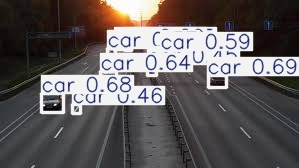
\includegraphics[width=0.9\columnwidth]{car_detections.jpg}
		\caption{Resultados da identificação de veículos utilizando um modelo pré-treinado do Ultralytics YOLO. As caixas delimitadoras indicam os veículos detectados com suas respectivas pontuações de confiança.}
		\label{fig:vehicle_detection}
	\end{center}
\end{figure}

\section{Conclusão}

Este artigo apresentou uma análise detalhada da aplicação da visão computacional, com foco na biblioteca Ultralytics YOLO, como uma solução robusta para desafios em engenharia e agricultura de precisão. A abordagem do YOLO, que reformula a detecção de objetos como um problema de regressão único, demonstrou ser altamente eficiente, oferecendo desempenho em tempo real com precisão satisfatória~\cite{Redmon2015}. A biblioteca Ultralytics YOLO destaca-se por sua versatilidade, suportando tarefas como detecção, segmentação, classificação, estimativa de pose e rastreamento de objetos, além de ser facilmente adaptável a diferentes plataformas de hardware, desde dispositivos periféricos até APIs na nuvem.

Os experimentos realizados, como a identificação de veículos em cenários urbanos apresentada na Fig.~\ref{fig:vehicle_detection}, evidenciaram a capacidade do modelo pré-treinado YOLOv11 de alcançar resultados robustos, especialmente em condições de boa iluminação, reforçando sua aplicabilidade em tarefas de monitoramento e automação. Além disso, a flexibilidade da biblioteca, com instalação simplificada via \texttt{pip} e suporte a treinamento personalizado, permite sua utilização em conjuntos de dados específicos, como os de agricultura de precisão, onde a análise de imagens de plantações de soja por VANTs pode otimizar o uso de recursos e maximizar a produtividade.

Apesar de limitações, como restrições espaciais e desafios na generalização para objetos com proporções incomuns, versões mais recentes, como o YOLOv8, introduzem melhorias significativas, como detecção sem âncoras e funções de perda avançadas, ampliando as possibilidades de aplicação~\cite{Redmon2015}. Assim, o Ultralytics YOLO consolida-se como uma ferramenta poderosa para a engenharia, oferecendo soluções práticas para monitoramento de infraestrutura, análise visual avançada e otimização de sistemas agrícolas, contribuindo para a sustentabilidade e eficiência em diversos domínios.


\bibliographystyle{IEEEtran}
\bibliography{bibliografia.bib}  % commented if *.bbl file included, as
%%%%%see below


%%%%%%%%%%%%%%%%% BIBLIOGRAPHY IN THE LaTeX file !!!!! %%%%%%%%%%%%%%%%%%%%%%%%
%% This is nothing else than the IEEEsample.bbl file that you would         
%%
%% obtain with BibTeX: you do not need to send around the *.bbl file        
%%
%%---------------------------------------------------------------------------%%

\end{document}
